\documentclass[fleqn, a4paper, 12pt, twoside]{article}
\usepackage{exsheets} %question and solution environments
\usepackage{amsmath, amssymb, amsthm} %standard AMS packages
\usepackage{esint} %integral signs
\usepackage{marginnote} %marginnotes
\usepackage{gensymb} %miscellaneous symbols
\usepackage{commath} %differential symbols
\usepackage{xcolor} %colours
\usepackage{cancel} %cancelling terms
\usepackage[free-standing-units]{siunitx} %formatting units
\usepackage{tikz, pgfplots} %diagrams
	\usetikzlibrary{calc, hobby, patterns, intersections, angles, quotes, spy}
\usepackage{graphicx} %inserting graphics
\usepackage{epstopdf} %converting and inserting eps graphics
\usepackage{hyperref} %hyperlinks
\usepackage{datetime} %date and time
\usepackage{ulem} %underline for \emph{}
\usepackage{xfrac, lmodern} %inline fractions
\usepackage{enumerate, enumitem} %numbered lists
\usepackage{float} %inserting floats
\usepackage[american voltages]{circuitikz} %circuit diagrams
\usepackage{pdflscape} %pages in landscape orientation
\usepackage{setspace} %double spacing
\usepackage{microtype} %micro-typography
\usepackage{listings} %formatting code
	\lstset{language=Matlab}
	\lstdefinestyle{standardMatlab}
	{
		belowcaptionskip=1\baselineskip,
		breaklines=true,
		frame=L,
		xleftmargin=\parindent,
		language=C,
		showstringspaces=false,
		basicstyle=\footnotesize\ttfamily,
		keywordstyle=\bfseries\color{green!40!black},
		commentstyle=\itshape\color{purple!40!black},
		identifierstyle=\color{blue},
		stringstyle=\color{orange},
	}
\usepackage{algpseudocode} %algorithms
\usepackage{algorithm} %algorithms
\usepackage{chronology}
\usepackage{qtree}
\usepackage{varwidth}
\usepackage{asymptote}

\newcommand\numberthis{\addtocounter{equation}{1}\tag{\theequation}} %adds numbers to specific equations in non-numbered list of equations

\theoremstyle{definition}
\newtheorem{example}{Example}
\newtheorem{definition}{Definition}

\theoremstyle{theorem}
\newtheorem{theorem}{Theorem}
\newtheorem{law}{Law}

\newcommand{\curl}{\mathrm{curl\,}}

\newcommand{\divergence}{\mathrm{div\,}}

\newcommand{\Arg}{\mathrm{Arg}}

\makeatletter
\@addtoreset{section}{part} %resets section numbers in new part
\makeatother

\newcommand\blfootnote[1]{%
	\begingroup
	\renewcommand\thefootnote{}\footnote{#1}%
	\addtocounter{footnote}{-1}%
	\endgroup
}

\renewcommand{\marginfont}{\scriptsize \color{blue}}

\renewcommand{\tilde}{\widetilde}

\SetupExSheets{solution/print = true} %prints all solutions by default

%opening
\title{Complex Functions}
\author{Aakash Jog}
\date{2015-16}

\begin{document}

\maketitle
%\setlength{\mathindent}{0pt}

\blfootnote
{	
	\begin{figure}[H]
		
\includegraphics[height = 12pt]{cc.eps}
		\includegraphics[height = 12pt]{by.eps}
		\includegraphics[height = 12pt]{nc.eps}
		\includegraphics[height = 12pt]{sa.eps}
	\end{figure}
	This work is licensed under the Creative Commons Attribution-NonCommercial-ShareAlike 4.0 International License. To view a copy of this license, visit \url{http://creativecommons.org/licenses/by-nc-sa/4.0/}.
} %CC-BY-NC-SA license

\tableofcontents

\newpage
\section{Lecturer Information}

\textbf{Zahi Hazan}\\
~\\
E-mail: \href{mailto:zahihaza@post.tau.ac.il}{zahihaza@post.tau.ac.il}\\

\section{Recommended Reading}

\begin{enumerate}
	\item James Ward Brown \& Ruel V. Churchill, ``Complex Variables and Applications'', McGraw-Hill, Inc. 1996.
	\item D. Zill, P. Shanahan, ``Complex Variables with Applications'', Jones and Bartlett Publishers.
\end{enumerate}

\section{Additional Reading}

\begin{enumerate}
	\item Saff, Edward B., and Arthur David Snider. Fundamentals of Complex Analysis with Applications to Engineering, Science, and Mathematics. 3rd ed. Upper Saddle River, NJ: Prentice Hall, 2002. ISBN: 0139078746.
	\item Sarason, Donald. Complex Function Theory. American Mathematical Society. ISBN: 0821886223
	\item Alfhors, Lars. Complex Analysis: An Introduction to the Theory of Analytic Functions of One Complex Variable. McGraw-Hill Education, 1979. ISBN: 0070006571.
\end{enumerate}

\newpage
\part{Complex Numbers}

\begin{definition}
	A number of the form
	\begin{align*}
		z & = x + i y
	\end{align*}
	where
	\begin{align*}
		i & = \sqrt{-1}    \\
		x & \in \mathbb{R} \\
		y & \in \mathbb{R}
	\end{align*}
	is called a complex number.
\end{definition}

\begin{definition}[Real part of a complex number]
	If
	\begin{align*}
		z & = x + i y
	\end{align*}
	then $x$ is called the real part of $z$, and is denoted as
	\begin{align*}
		x & = \Re(z)
	\end{align*}
\end{definition}

\begin{definition}[Imaginary part of a complex number]
	If
	\begin{align*}
		z & = x + i y
	\end{align*}
	then $y$ is called the imaginary part of $z$, and is denoted as
	\begin{align*}
		x & = \Im(z)
	\end{align*}
\end{definition}

\begin{definition}[Complex conjugate]
	If
	\begin{align*}
		z & = x + i y
	\end{align*}
	then
	\begin{align*}
		\overline{z} & = x - i y
	\end{align*}
	is called the complex conjugate of $z$.
\end{definition}

\begin{theorem}
	\begin{align*}
		z \overline{z} & = |z|^2
	\end{align*}
\end{theorem}

\begin{proof}
	\begin{align*}
		z                       & = x + i y \\
		\therefore \overline{z} & = x - i y
	\end{align*}
	Therefore,
	\begin{align*}
		z \overline{z} & = (x + i y) (x - i y)       \\
                               & = x^2 - i x y + i x y + y^2 \\
                               & = x^2 + y^2                 \\
                               & = |z|^2
	\end{align*}
\end{proof}

\begin{definition}[Polar representation]
	If
	\begin{align*}
		x & = r \cos \theta \\
		y & = r \sin \theta
	\end{align*}
	then $(r,\theta)$ is called the polar representation of $(x,y)$.
\end{definition}

\begin{theorem}[Euler's Formula]
	\begin{align*}
		r cos \theta + i r \sin \theta & = r e^{i \theta}
	\end{align*}
	\label{Euler's_Formula}
\end{theorem}

\begin{definition}[Absolute value or Norm]
	\begin{align*}
		|z| & = |x + i y| \\
                    & = \sqrt{x^2 + y^2}
	\end{align*}
	is called the absolute value, or the norm of $z$.
\end{definition}

\begin{theorem}
	\begin{equation*}
		|z| \le \left| \Re(z) \right| + \left| \Im(z) \right| \le \sqrt{2} |z|
	\end{equation*}
\end{theorem}

\begin{proof}
	\begin{gather*}
		\sqrt{x^2 + y^2} \le |x| + |y| \le \sqrt{2 x^2 + 2 y^2}\\
		\iff x^2 + y^2 \le x^2 + y^2 + 2 |x| |y| \le 2 x^2 + 2 y^2\\
		\iff x^2 + y^2 - 2 |x| |y| \ge 0\\
		\iff \left( |x| - |y| \right)^2 \ge 0
	\end{gather*}
\end{proof}

\begin{definition}[Argument]
	Let $z$ be a complex number.\\
Then, $\theta$, such that $\theta \in (-\pi,\pi]$, and
	\begin{align*}
		z & = (r,\theta)
	\end{align*}
	is called the argument of $z$.\\
	It is denoted as
	\begin{align*}
		\theta & = \Arg(z)
	\end{align*}
	If $\theta \notin (-\pi,\pi]$, but
	\begin{align*}
		z & = (r,\theta)
	\end{align*}
	then
	\begin{align*}
		\theta & = \arg(z)
	\end{align*}
\end{definition}

\begin{theorem}
	\begin{align*}
		z^n & = |z|^n e^{i n \Arg(z)}
	\end{align*}
\end{theorem}

\begin{proof}
	\begin{align*}
		z              & = |z| e^{i \Arg(z)}                                   \\
		\therefore z^n & = \left( |z| e^{i \Arg(z)} \right)^n                  \\
                               & = \left( |z| \right)^n \left( e^{i \Arg(z)} \right)^n \\
                               & = |z|^n e^{i n \Arg(x)}
	\end{align*}
\end{proof}

\begin{theorem}
	Let
	\begin{align*}
		z & = r e^{i \theta} \\
		w & = \rho e^{i \varphi}
	\end{align*}
	The solutions to
	\begin{align*}
		w & = \sqrt[n]{z}
	\end{align*}
	are
	\begin{align*}
		\varphi_k & = \frac{\theta}{n} + \frac{2 \pi k}{n}
	\end{align*}
	where $k \in \{0,\dots,n - 1\}$.
\end{theorem}

\begin{proof}
	\begin{align*}
		w              & = \sqrt[n]{z} \\
		\therefore w^n & = z
	\end{align*}
	Therefore,
	\begin{align*}
		\rho^n e^{i n \varphi} & = r e^{i \theta}
	\end{align*}
	Therefore, for $k \in \{0,\dots,n - 1\}$,
	\begin{align*}
		\rho               & = \sqrt[n]{r}      \\
		n \varphi          & = \theta + 2 \pi k \\
		\therefore \varphi & = \frac{\theta}{n} + \frac{2 \pi k}{n}
	\end{align*}
\end{proof}

\newpage
\part{Complex Sequences and Series}

\begin{definition}[Convergence of complex sequences]
	Let
	\begin{align*}
		z_n & = x_n + i y_n
	\end{align*}
	The sequence $\{z_n\}$ is said to converge to the limit $z = x + i y$, if $\forall \varepsilon > 0$, $\exists N$, such that $\forall n > N$, $|z_n - z| < \varepsilon$, i.e. there is a circular region of radius $\varepsilon$, centred at $z$, in which $z_n$ lies.
\end{definition}

\begin{theorem}
	$\{z_n\} \to z$, i.e. $\{z_n\}$ converges to $z$ if and only if all subsequences of $\{z_n\}$ converge to $z$.
\end{theorem}

\newpage
\part{Topology on the Complex Plane}

\begin{definition}[Neighbourhood of a complex number]
	A circular region of radius $\varepsilon$ centred at $z$, is called the $\varepsilon$ neighbourhood of $z$.
	\begin{align*}
		B(z,\varepsilon) & = \left\{ w \in \mathbb{C} : |w - z| < \varepsilon \right\}
	\end{align*}
	\begin{figure}[h]
		\centering
		\begin{tikzpicture}
			\def\xMIN{-1};
			\def\xMAX{4};
			\def\yMIN{-1};
			\def\yMAX{4};
	
			\coordinate (z) at (2,2);
	
			\def\epsilon{0.8};
	
			\begin{scope}[stealth-stealth]
				\draw (\xMIN,0) -- (\xMAX,0) node [right] {$\Re$};
				\draw (0,\yMIN) -- (0,\yMAX) node [above] {$\Im$};
			\end{scope}
	
			\begin{scope}
				\draw [fill = lightgray] (z) circle (\epsilon);
	
				\draw [-stealth] (z) -- ++(30:\epsilon) node [midway, below] {$\varepsilon$};
			\end{scope}

			\begin{scope}
				\draw (z) circle (1pt) node [below] {$z$};
			\end{scope}
		\end{tikzpicture}
		\caption{Neighbourhood of a complex number}
	\end{figure}
\end{definition}

\begin{definition}[Inner point]
	Let $A \subseteq \mathbb{C}$.\\
	$z \in \mathbb{C}$ is called an inner point of $A$ if there exists at least one $\varepsilon_z > 0$, such that $B(z,\varepsilon_z) \subset A$.
\end{definition}

\begin{definition}[Outer point]
	Let $A \subseteq \mathbb{C}$.\\
	$z \in \mathbb{C}$ is called an outer point of $A$ if there exists at least one $\varepsilon_z > 0$, such that $B(z,\varepsilon_z) \subset (\mathbb{C} \setminus A)$.
\end{definition}

\begin{definition}[Edge point]
	Let $A \subseteq \mathbb{C}$.\\
	$z \in \mathbb{C}$ is called an edge point of $A$ if it is neither an inner point of $A$, nor an outer point of $A$.
\end{definition}

\end{document}
